\documentclass[conference]{IEEEtran}
\IEEEoverridecommandlockouts
% The preceding line is only needed to identify funding in the first footnote. If that is unneeded, please comment it out.
\usepackage{cite}
\usepackage{amsmath,amssymb,amsfonts}
\usepackage{algorithmic}
\usepackage{graphicx}
\usepackage{textcomp}
\usepackage{xcolor}
\def\BibTeX{{\rm B\kern-.05em{\sc i\kern-.025em b}\kern-.08em
    T\kern-.1667em\lower.7ex\hbox{E}\kern-.125emX}}

\makeatletter
\def\endthebibliography{%
  \def\@noitemerr{\@latex@warning{Empty `thebibliography' environment}}%
  \endlist
}
\makeatother


\begin{document}

\title{SplitterGUI\\
{\large GUI Application of Mining Fine-Grained Sequential Patterns in Semantic Trajectories}
\thanks{The SplitterGUI project files can be downloaded at
$github.com/dzakybd/Datastream-project$}
}

\author{\IEEEauthorblockN{Tanjung Dion, Fawwaz Dzaky Zakiyal}
\IEEEauthorblockA{\textit{Department of Electrical and Computer Engineering} \\
\textit{Pusan National University}\\
Busan, Republic of Korea \\
\{tanjung.dn, dzakybd\}@gmail.com}}

\maketitle

\begin{abstract}
Semantic trajectory is a sequence of timestamped places wherein each place has information about spatial location and a semantic label. By mining fine-grained pattern that satisfy semantic consistency, spatial compactness and temporal continuity, it will give benefit such as urban planning and targeted advertising. One of the state-the-art method to mine the fine-grained pattern is Splitter algorithm. Firstly, it find set of coarse patterns and their snippets by using PrefixSpan, and then find the set of fine-grained patterns using mean shift method. In this project we build, SplitterGUI, GUI application to visualize the process of the Splitter algorithm. We also discuss the key techniques in Splitter and conduct an experiment using 4SQ database to demontrate the result of SplitterGUI.

\end{abstract}

\begin{IEEEkeywords}
fine-grained pattern, semantic trajectories, GUI application.
\end{IEEEkeywords}

\section{Introduction}
The sequential patterns can be found in a trajectory database, if it properly extracted. It become benefit for targeted advertising, urban planning, location prediction, etc. In other hand, classic sequential pattern mining algorithms cannot work effectively in semantic trajectories, a sequence of time-stamped places wherein each place has information about spatial location and a semantic label. Because of the places in the continuous space cannot be regarded as independent items, so independent place cannot be used to find the frequent sequences. Instead, semantic label need to be grouped to form frequent sequential patterns. But, there is also a challenge to get fine-grained sequential patterns, that it must fulfill requirements of spatial compactness (compact area for each place category), semantic consistency (consistent place ID in each place category) and temporal continuity (limited time constraint).
\par
The process of mining fine-grained pattern have been proposed by Zang et. al \cite{zhang2014splitter}. They provide two-step approach to obtain fine-grained sequential patterns. First-step, obtain the coarse patterns from the semantic trajectory data using the full projection method to modify PrefixSpan. The result patterns will fullfil the semantic and temporal constraints. Second-step, splitting each coarse patterns into fine-grained patterns that fulfill the spatial constraint through top-down pattern discovery process using weighted snippet shift by Epanechnikov kernel.
\par
In this project, aiming at implementing the mining fine-grained pattern method proposed by Zang et. al \cite{zhang2014splitter} and build the GUI application to visualize the process of the Splitter algorithm, called SplitterGUI. It make the database, course patterns and fine-grained patterns into a visualized map by determined Splitter algoritm's parameters. Afterwards, we discuss the key techniques in Splitter and conduct an experiment using 4SQ database to demontrate the result of SplitterGUI.


\section{Implementation}
\subsection{System Design}
\begin{figure}[!ht]
\centering
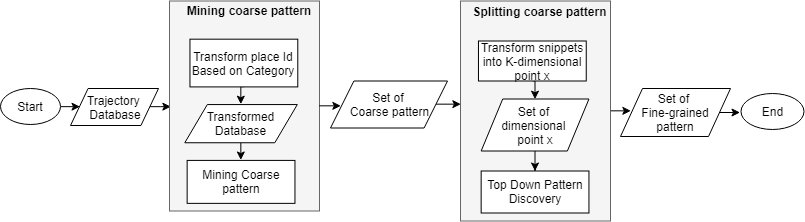
\includegraphics[width=0.55\linewidth]{splitter}
\caption{System Design}
\label{fig:systemdesign}
\end{figure}
Figure \ref{fig:systemdesign} show the process of mining fine-grained pattern in semantic trajectories. This method consist of two part: mining coarse pattern and splitting coarse pattern. Mining coarse pattern is a process to find sequential pattern that satisfy semantic consistency and temporal continuity. In the first step, we add trajectory database that have information about place id, movement time, group id, and spatial location to the system. This trajectory database will be transformed into semantic trajectory database by grouping place id based on category. However, we still keep the original place id in each category to prevent one trajectory from being counted repeatedly. By doing this process, our trajectory database will satisfy semantic consistency.
\par
Then, PrefixSpan algorithm will be used to mining the coarse pattern. In the PrefixSpan algorithm, we include all post-fixes to avoid missing pattern under the given time constrain. Output from mining coarse pattern is set of coarse pattern that will be used in the next process. The next process is finding fine-grained pattern that satisfy spatial compactness in by splitting a coarse pattern in top down manner. Set of coarse pattern from previous process will be transformed into K-dimensional point x.
\par
Then, we employ mean shift clustering to extract the dense and compact snippet cluster based on the support and variance threshold. To speed up the process, the unqualified snippet cluster will be organized into several disjoint communities. By only clustering each communities, we can gradually reduce the kernel windows in clustering method to speed up the clustering process.

\subsection{Key techniques in Splitter}
\subsubsection{Mining Coarse Pattern}
Before mining coarse pattern, trajectory database D should be transformed to semantic trajectory by grouping each place based on its category. The purpose is to find any frequent sequences that have similar categories. For example, Fig. \ref{fig:transformed-database} shows database transformation with office $=G_{1}$, shop $=G_{2}$, restaurant $=G_{3}$. 

\begin{figure}[!ht]
	\centering
	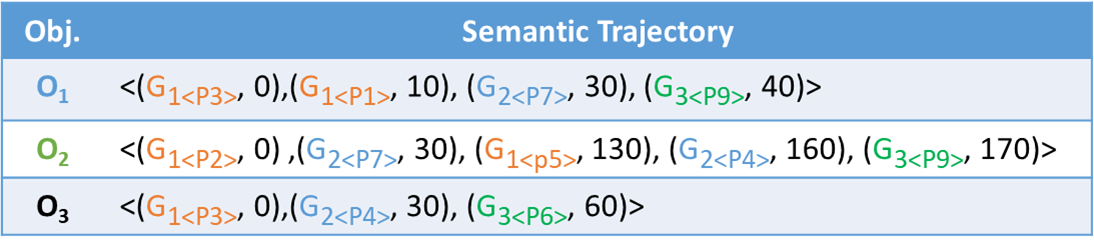
\includegraphics[width=1\linewidth]{transformed_database}
	\caption{Semantic trajectory database}
	\label{fig:transformed-database}
\end{figure}

After transformation, we mining sequential pattern that satisfy support threshold $\sigma$ and time constraint $\Delta t$ using PrefixSPan algorithm. PrefixSpan algorithm use frequent item as short pattern and prefixes to build projected database then grow the short pattern by searching local frequent item in projected database. However, PrefixSpan algorithm should be modified to satisfy our coarse pattern. \ref{fig:mining-coarse-pattern} shows the modified prefix span algorithm. First, we extract all frequent item at least $\sigma$ in semantic trajectory D. Then for each item we build item-projected database as S using full projection. Full projection means that we extract all pattern that occurred in database. For example, object 0 in \ref{fig:transformed-database} has 2 pattern $P_{3}\rightarrow P_{7}\rightarrow P_{9}$ and $P_{1}\rightarrow P_{7}\rightarrow P_{9}$.
\par
Output this item as our short pattern and then grow this pattern by calling PrefixSpan function. This function has similar procedure with initial projection function. However, we check time constraint when searching frequent item in projected database. We also call this PrefixSpan function recursively to grow the pattern until the pattern cannot be grown anymore. Output of this algorithm is list of coarse pattern with its snippet (i.e. $P_{1}\rightarrow P_{7}\rightarrow P_{9}$), group (i.e. $G_{1}\rightarrow G_{2}\rightarrow G_{3}$), and pattern length (i.e. 3).  

\begin{figure}[!ht]
	\centering
	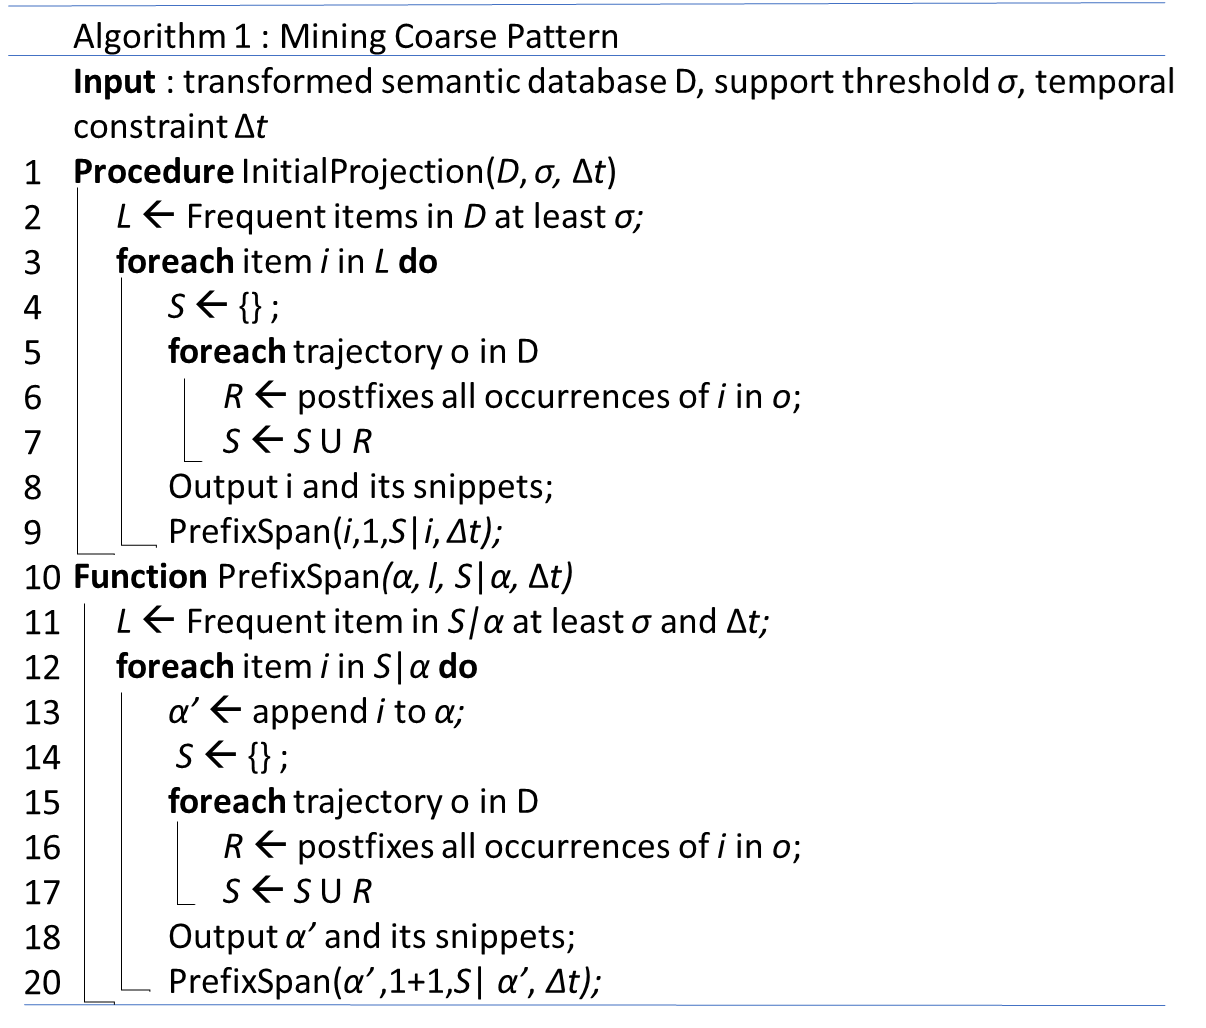
\includegraphics[width=1.0\linewidth]{mining_coarse_pattern}
	\caption{Mining coarse pattern algorithm}
	\label{fig:mining-coarse-pattern}
\end{figure}

\subsubsection{Finding Fine-Grained Pattern}
The result of coarse pattern has satisfy support threshold $\sigma$ and time constraint $\Delta t$. Next step is checking the spatial variance of place in each group category. For example, graph representation of coarse pattern is shown in Fig. \ref{fig:graph-coarse-pattern}. Spatial location of place $P_{5}$ with other place in group $G_{1}$ is to far. Therefore, we have to prune pattern $P_{5}\rightarrow P_{4}\rightarrow P_{6}$ from fine-grained pattern. 
\begin{figure}[!ht]
	\centering
	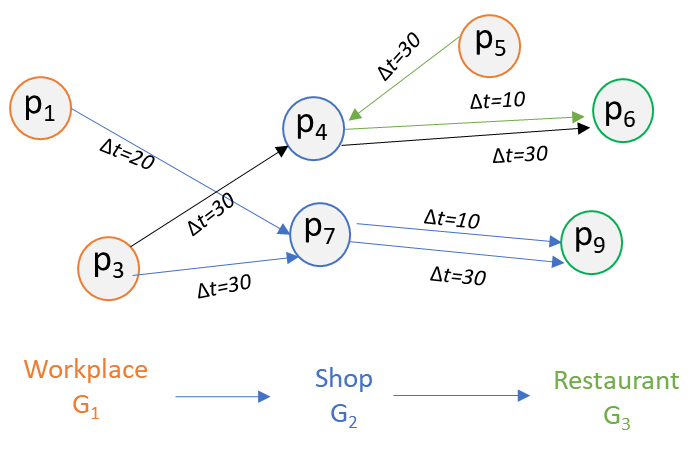
\includegraphics[width=0.7\linewidth]{graph_coarse_pattern}
	\caption{Graph representation of coarse pattern result}
	\label{fig:graph-coarse-pattern}
\end{figure}
For finding fine-grained pattern, mean shift clustering algorithm is used because it does not need any prior knowledge and only use one parameter called bandwidth. Bandwidth parameter is used to limit the area of clustering. The main idea of mean shift algorithm is choosing random point as the center and use bandwidth to limit the coverage area of clustering. Then calculate mean shift vector to shift the center point toward new point that more dense than previous point. 

\section{Demonstration}

\subsection{Database}
This project will use the real database, 4SQ that collected from Foursquare check-in sequence in New York. It consists of 48564 places that divided into 417 place categories and it stored semantic trajectories from 14909 users. 4SQ database provides 3 files:
\begin{enumerate}
\item \textit{Sequences}, it contains users semantic trajectories including attributes of check-in time-stamp and place ID.
\item \textit{Places}, it contains information about the places (place ID, latitude, longitude, category ID).
\item \textit{Category}, it contains information of place category ID corresponding with its place category name.
\end{enumerate}

\subsection{Result}
We will re-implement the process of mining fine-grained pattern using java programing language. The user interface of program will be provided as shown in the Figure. Figure shows the illustration of our program. There are an database input in csv format, 4 parameters input,  show button for showing graph representation like in the figure, and 3 button to start the process individually or start all of the process respectively.

\section*{Acknowledgment}
This paper is submitted to fulfill term project task from Stream Database class (Fall 2018), Pusan National University.

\bibliographystyle{IEEEtran}
\bibliography{refs}

\end{document}
